\documentclass[UTF8,11pt,a4paper]{ctexart}
\usepackage[a4paper,margin=2.4cm]{geometry}
\usepackage{amsmath,amssymb,amsthm,booktabs,enumitem,graphicx,xcolor,microtype}
\usepackage{hyperref}
\hypersetup{colorlinks=true,linkcolor=blue,citecolor=blue,urlcolor=blue}
\theoremstyle{plain}
\newtheorem{theorem}{定理}
\newtheorem{lemma}[theorem]{引理}
\setlist{nosep,leftmargin=*}
\setlength{\emergencystretch}{3em}
\graphicspath{{../../figures/}{figures/}}

\title{从结构稳定性到结构迁移：大语言模型推理中的结构因素}
\author{}
\date{实验前研究正文草稿}

\begin{document}
\maketitle

\begin{abstract}
大语言模型在多步推理任务上取得了较高准确率，但模型在同一道题的不同呈现方式下能否保持正确，以及模型能否迁移到未见的依赖结构，是两个不应混为一谈的问题。本文将前者定义为结构稳定性，将后者定义为结构迁移，并在符号层面构造相互独立的测量数据池。结构稳定性使用同一依赖图上的条件保持率，结构迁移使用已见图族与未见图族在规范呈现下的性能差距。进一步地，本文提出以相关前提距离、活动依赖前沿和算子协调数为核心的依赖负担错误规律，并通过发现集、确认集、第二任务族和匹配训练干预检验其样本外预测能力与适用边界。StructShift 仅作为求解器验证的测量模块，LoRA 仅作为后续边界干预。本文为实验前研究设计，不包含实证数量结论。
\end{abstract}

\section{引言}

大语言模型能够处理数学、逻辑和知识密集型多步推理任务。然而，模型在随机划分上的高准确率并不能回答两个不同的问题：第一，模型已经解决的问题换一种合法呈现方式后是否仍然能够保持正确；第二，模型能否将熟悉的局部操作组合到训练中没有出现过的新依赖结构中。前者反映已获得能力的稳定发挥，后者反映结构组合和系统性迁移。若将二者统称为结构鲁棒性或结构外推能力，就无法判断错误究竟来自基础能力不足、呈现脆弱性还是新结构组合失败。

组合泛化研究已经表明，模型可能掌握任务部件，却无法稳定迁移到未见组合[1--4]。数学推理与上下文干扰研究也显示，受控实例化、无关子句和信息位置会影响模型输出[5--8]。但是，这些设置改变的对象并不相同：有的改变任务图，有的改变表面形式，有的插入干扰信息，有的改变中间解释。如果不对这些因素进行分离，准确率下降便不能被准确解释。

本文提出一条分层研究路线。首先，在同一依赖图上生成答案保持的前提重排和语义等价呈现，测量模型能否保持已经展示出的正确答案。其次，在独立数据池中留出图族或算子组合，测量模型能否迁移到新的依赖结构。再次，利用求解器轨迹计算相关前提距离和活动依赖前沿，建立一个在发现集上确定、在确认集上检验的错误预测规律。最后，在第二个任务族以及匹配训练干预中检验这一规律的边界。

本文的计划贡献包括：\textbf{(1)} 给出不循环的结构稳定性与结构迁移定义；\textbf{(2)} 构造求解器验证、数据池独立的测量协议；\textbf{(3)} 提出可被样本外数据推翻的依赖负担错误规律；\textbf{(4)} 通过独立任务和匹配干预报告规律的适用边界。当前稿件不声称任何实证结果。

\begin{figure}[t]
  \centering
  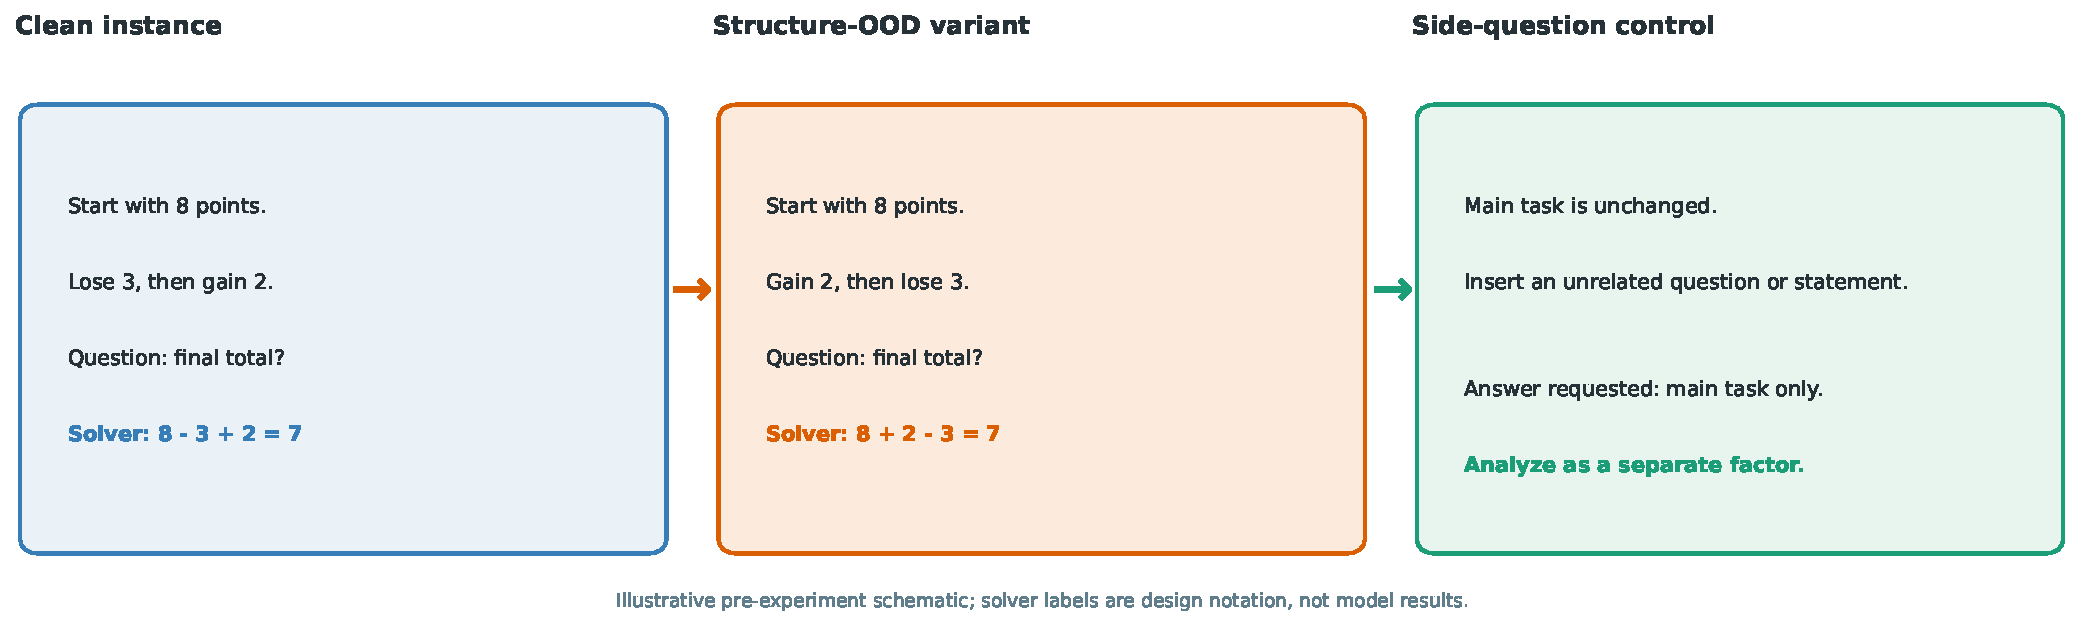
\includegraphics[width=\linewidth]{fig1_motivated_example.pdf}
  \caption{同一依赖图的规范呈现和等价变体。正式图中将进一步标出独立迁移池中的未见图样本。}
  \label{fig:motivation-zh}
\end{figure}

\section{相关工作}

\paragraph{组合泛化。} 组合泛化研究关注模型能否将熟悉部件系统地组合到未见结构中[1--4]。本文借鉴结构留出的思想，但将研究对象放在最终答案推理，并把同图呈现稳定性与新图结构迁移分开测量。

\paragraph{推理鲁棒性与上下文干扰。} GSM-Symbolic 和 GSM-Plus 等工作考察数学实例、附加子句和相关扰动[5,6]；其他研究分析无关上下文和信息位置[7,8]。本文将 decoy 和 side-question 作为干扰分析池，不把它们直接等同于新依赖结构。

\paragraph{思维链与忠实性。} 噪声思维链和忠实性研究改变中间解释或检验解释是否支持答案[9,10]。本文的主要对象是输入任务结构，不能仅依据输出答案推断模型内部推理机制。

\paragraph{参数高效适配。} LoRA 与 QLoRA 提供参数高效适配机制[13,14]，目标化对抗训练通过当前错误选择训练样本[15]。本文只把它们用于匹配预算下的边界干预。

\section{结构稳定性与结构迁移}

\subsection{问题表示}

将一个潜在推理任务表示为 $z=(G,q,y)$，文本呈现记为 $r$，模型实际看到的输入为
\begin{equation}
x=R(z,r).
\end{equation}
其中 $G$ 是符号依赖图，$q$ 是目标问题，$y$ 是求解器验证的答案。该表示把潜在任务与表面呈现分开。

\subsection{结构稳定性}

稳定性变换 $T_s$ 只能改变呈现方式，并满足
\begin{equation}
G(T_sx)=G(x),\qquad q(T_sx)=q(x),\qquad y(T_sx)=y(x).
\end{equation}
由于变体准确率同时包含基础能力和呈现稳定性，本文使用原题答对条件下的保持率：
\begin{equation}
SS(f)=\Pr[f(T_sx)=y\mid f(x)=y],
\qquad
SF(f)=1-SS(f).
\end{equation}
$SS(f)$ 衡量模型已经展示出解题能力后，是否能够在等价呈现下保留正确答案。
为检查条件化本身的影响，补充报告同一任务的两个随机等价呈现的一致率
\begin{equation}
INV(f)=\mathbb E_{z,r,r'}\left[
\mathbf 1\{f(R(z,r))=f(R(z,r'))\}\right].
\end{equation}
若模型稳定地犯同一种错，$INV$ 仍可能很高而 $SS$ 很低。

\subsection{结构迁移}

迁移池包含发现阶段和稳定性池中没有出现过的图族或算子组合。这里不再固定单个潜在任务，而是比较已见图分布 $P_S(G)$ 与未见图分布 $P_U(G)$ 上的风险：
\begin{equation}
R_S(f)=\mathbb E_{G\sim P_S,q\sim P(q\mid G)}
\left[\mathbf 1\{f(x_G^{\mathrm{can}})\neq y_G\}\right],
\end{equation}
\begin{equation}
R_U(f)=\mathbb E_{G\sim P_U,q\sim P(q\mid G)}
\left[\mathbf 1\{f(x_G^{\mathrm{can}})\neq y_G\}\right].
\end{equation}
规范呈现下的迁移差距定义为
\begin{equation}
\Delta_T(f)=
\Pr_{G\sim P_{\mathrm{seen}}}[f(x_G^{\mathrm{can}})=y_G]
-\Pr_{G\sim P_{\mathrm{unseen}}}[f(x_G^{\mathrm{can}})=y_G].
\end{equation}
两个图分布使用匹配的基础算子、长度、标签和模板条件。$\Delta_T(f)$ 衡量模型从已见图族迁移到未见图族时的性能变化，而不是同一图的呈现变化。
等价地，$\Delta_T=R_U-R_S$，是图分布支持变化带来的风险增量。可补充报告归一化迁移保留率
\begin{equation}
TR(f)=1-\frac{R_U(f)-R_S(f)}{1-R_S(f)},\qquad R_S<1.
\end{equation}
因此，稳定性是在固定 $z$ 后比较呈现，迁移是在固定规范呈现后比较两个 $G$ 分布；两者不是同一个量。

\subsection{二乘二分解}

令 $A_{g,p}$ 表示图熟悉度 $g\in\{\mathrm{seen},\mathrm{unseen}\}$ 和呈现方式 $p\in\{\mathrm{canonical},\mathrm{shifted}\}$ 下的准确率。稳定性差距、迁移差距和交互效应分别为
\begin{equation}
\Delta_S=A_{\mathrm{seen,canonical}}-A_{\mathrm{seen,shifted}},
\end{equation}
\begin{equation}
\Delta_T=A_{\mathrm{seen,canonical}}-A_{\mathrm{unseen,canonical}},
\end{equation}
\begin{equation}
I_{S\times T}=
\left(A_{\mathrm{seen,canonical}}-A_{\mathrm{seen,shifted}}\right)
-\left(A_{\mathrm{unseen,canonical}}-A_{\mathrm{unseen,shifted}}\right).
\end{equation}
三个量具有不同的数据支持和比较方向，因而不将稳定性和迁移视为同一个指标。

\subsection{闭包求解器上的有限定理}

下列陈述在 Lean~4 中证明，证明见附录~\ref{app:proofs-zh}。它们只约束闭包求解器和有限反例，不是对已训练模型的实测结论。原子取自然数。一条规则写成前提集推出结论。求解器答案记为 $y$。顺序、同义、删前提、换图分别记为 $O_\sigma$、$L^{\equiv}$、$L^{\times}$、$H_\psi$。抽取记为 $\varphi$。闭包求解器是
\begin{equation}
f(x)=\mathbf{1}\{q\in\mathrm{Closure}(\varphi(x))\},
\end{equation}
并且对一切稳定性变换 $T_s$ 有 $\varphi(T_sx)=\varphi(x)$。燃料不少于规则条数时，闭包成员关系与确定子句推导一致。

\begin{lemma}[顺序与同义]
\label{lem:order-zh}
\begin{align}
y(O_\sigma\omega)&=y(\omega),\\
y(L^{\equiv}\omega)&=y(\omega).
\end{align}
因而 $O_\sigma$ 与 $L^{\equiv}$ 是稳定性变换。取事实集为空、规则 $\{0\}\to 1$、查询 $1$ 的任务 $\omega_0$，则
\begin{equation}
y(\omega_0)=\mathrm{no},\qquad y(L^{\times}\omega_0)=\mathrm{yes},
\end{equation}
故 $L^{\times}$ 不是稳定性变换。$H_\psi$ 把 $\{0\}\to 1$ 换成 $\{0\}\to 2$，两个规则集不相等，因而也不是稳定性变换。
\end{lemma}

\begin{lemma}[准确率之差与改口计数]
\label{lem:gap-zh}
设每条观测的 $C,S\in\{0,1\}$。在任意有限列表上，
\begin{equation}
\#\{C=1\}-\#\{S=1\}=\#\{C=1,S=0\}-\#\{C=0,S=1\}.
\end{equation}
记 $\Delta=\#\{C=1\}-\#\{S=1\}$，$N=\#\{C=1\}$，$F=\#\{C=1,S=0\}$，$R=\#\{C=0,S=1\}$。则
\begin{equation}
\Delta\cdot N=FN-RN,
\qquad
SF=\frac{F}{N}\quad(N>0).
\end{equation}
因此 $\Delta=0$ 不推出 $F=0$。反例是两个长度为 $100$ 的列表，都有 $N=60$，而
\begin{equation}
SF\in\left\{0,\frac{30}{60}\right\}.
\end{equation}
\end{lemma}

\begin{lemma}[见过图上的改口与换图差距]
\label{lem:worlds-zh}
两个长度为 $2$ 的有限世界 $W_{=}$ 与 $W_{\neq}$ 满足
\begin{equation}
\#_{\mathrm{seen}}\{C=1\}=\#_{\mathrm{unseen}}\{C=1\}=2,
\qquad
\Delta_T(W_{=})=\Delta_T(W_{\neq})=0,
\end{equation}
而见过图上的改口次数为
\begin{equation}
F(W_{=})=0,\qquad F(W_{\neq})=1.
\end{equation}
\end{lemma}

\begin{lemma}[交互与呈现差互为相反数]
\label{lem:interaction-zh}
在整数上，
\begin{align}
I_{S\times T}
&=(A_{\mathrm{sc}}-A_{\mathrm{ss}})-(A_{\mathrm{uc}}-A_{\mathrm{us}}),\\
J
&=(A_{\mathrm{ss}}-A_{\mathrm{us}})-(A_{\mathrm{sc}}-A_{\mathrm{uc}}),
\end{align}
并且
\begin{equation}
I_{S\times T}=-J.
\end{equation}
\end{lemma}

\begin{lemma}[倒序的逆序对]
\label{lem:inversion-zh}
\begin{equation}
\operatorname{inv}(\mathrm{rev}(m))=\frac{m(m-1)}{2},
\qquad
\operatorname{inv}(\mathrm{id})=0.
\end{equation}
因此
\begin{equation}
\operatorname{inv}(\mathrm{rev}(2))=1\neq 3=\operatorname{inv}(\mathrm{rev}(3)).
\end{equation}
这是组合恒等式，不是实验测量。
\end{lemma}

\begin{theorem}[闭包求解器的轨道与一个反例函数]
\label{thm:main-zh}
若 $\varphi\circ O_\sigma=\varphi$ 且 $\varphi\circ L^{\equiv}=\varphi$，则在该轨道上
\begin{equation}
f(x)=y\implies f(T_sx)=y,
\end{equation}
即 $SS(f)=1$。若没见过的图仍被正确抽取，则
\begin{equation}
f(x_U^{\mathrm{can}})=y
\qquad\text{且}\qquad
f(T_sx_U)=y.
\end{equation}
反支取见过写法 $\mathrm{seen}(t)$，$t\in\mathbb{N}$，规则 $\{0\}\to 1$，事实 $\{0\}$，查询 $1$；没见过的规范写法规则为 $\emptyset\to 2$，事实为空，查询 $2$。两个规则集不相交，求解器在两处都回答 $\mathrm{yes}$。存在函数
\begin{equation}
g(\mathrm{seen}(t))=\mathrm{yes},
\qquad
g(x_U^{\mathrm{can}})=\mathrm{no}.
\end{equation}
于是 $g$ 在见过图的全部写法上稳定且正确，在该没见过题上不正确。只在见过写法上得到支持的重排训练排除不了 $g$。
\end{theorem}

\section{依赖负担错误规律}

本文考察一个任务层面的候选解释：模型的一部分错误来自依赖跟踪负担，而不仅仅来自输入长度。令 $D_{\mathrm{rel}}(x)$ 表示证明所需前提之间的距离，$F_{\mathrm{active}}(x)$ 表示最多同时保持活动的未完成依赖数量，则候选模型为
\begin{equation}
\operatorname{logit}\Pr(e_{m,x}=1)
=\alpha_m+\beta_1D_{\mathrm{rel}}(x)
+\beta_2F_{\mathrm{active}}(x)+\gamma^\top Z(x),
\end{equation}
其中 $Z(x)$ 控制总长度、图规模、目标位置、模板、标签、深度和分支数。模型规格和系数方向在发现集上确定，并在确认集上比较 held-out log loss、Brier score、校准和负担区间错误率。

在二乘二数据上，进一步加入呈现变化和未见图指标：
\begin{equation}
\operatorname{logit}\Pr(e_{m,x}=1)
=\alpha_m+\eta_S I_{\mathrm{shift}}(x)
+\eta_T I_{\mathrm{unseen}}(x)
+\eta_{ST}I_{\mathrm{shift}}(x)I_{\mathrm{unseen}}(x)
+\beta^\top X(x).
\end{equation}
$\eta_S$、$\eta_T$ 和 $\eta_{ST}$ 分别表示稳定性、迁移和交互效应。该模型不把两个指标合并，而是检验它们是否产生不同的错误增量。

\subsection{具体规律与可证伪预测}

本文不把三个结构特征与错误的相关性直接称为规律，而是先构造标准化依赖负担分数
\begin{equation}
B(x)=w_D\widetilde D_{\mathrm{rel}}(x)
+w_F\widetilde F_{\mathrm{active}}(x)
+w_K\widetilde K_{\mathrm{op}}(x),
\qquad w_D,w_F,w_K\geq 0.
\end{equation}
依赖负担规律写成条件错误风险
\begin{equation}
\Pr(e_{m,x}=1\mid B(x),Z(x))
=\sigma\left(\alpha_m+\phi(B(x))+\gamma^\top Z(x)\right),
\end{equation}
其中 $Z(x)$ 控制长度、图规模、深度、分支、目标位置和模板，$\phi$ 在工作区间内单调不减。主模型使用线性 $\phi$，单调样条用于形状检查。

该规律的可证伪预测是：控制 $Z$ 后，$B$ 更高的题应有更高错误风险；依赖负担模型应优于最强长度/图规模对照；按负担分箱后的错误率应单调增加。方向反转、预测优势消失、分箱不单调或 placebo 提示同样有效，都只能支持探索性趋势。

如果局部子问题和完整问题同样容易错，或者只用长度和图规模的模型预测同样准确，则不能把依赖负担规律写成确认性解释。正确依赖提示与格式匹配的 placebo 提示也用于排除一般提示效应。

\section{实验设计}

\subsection{E1：结构稳定性}

在同一依赖图上生成规范呈现、合法前提重排、语义等价模板和长度匹配的相关前提距离变化。增加深度、增加分支和改变算子组合不放入稳定性定义。报告原题准确率、变体准确率、条件保持率、条件翻转率和按 base query 配对的 bootstrap 区间。

\subsection{E2：结构迁移}

在符号层切分独立的未见图族和未见算子组合，并使用规范呈现评估迁移。稳定性和迁移不能共享 world、base query、图哈希或图族。只有在多个模型、checkpoint 或受控训练条件上，才分析稳定性对迁移的预测关系，并控制独立测得的 clean competence。

\subsection{E2.5：正交干预的双重分离}

设置 Base、Render-Aug、Graph-Aug 和 Joint 四种匹配训练条件。Render-Aug 只扩充同图的等价呈现，Graph-Aug 只扩充 canonical 呈现下的新图组合，Joint 同时扩充两者。四个条件均在二乘二四格上评估，并匹配训练 token、步数、LoRA rank、目标模块、随机种子和计算预算。

相对 Base 的收益定义为
\begin{equation}
G_S(c)=SS_c-SS_{\mathrm{Base}},\qquad
G_T(c)=\Delta_{T,\mathrm{Base}}-\Delta_{T,c}.
\end{equation}
只有当 Render-Aug 显著提高 $G_S$ 且 $G_T$ 落入预注册的迁移等价界限内，才支持主要改善稳定性；Graph-Aug 的判定反过来。双重分离需要等价检验或置信区间，不能用一个显著、另一个不显著来替代。

\subsection{E3：样本外错误预测}

在 discovery split 上选择依赖特征、交互项、随机效应和对照模型，在 confirmatory split 上冻结检验。比较长度模型、图规模模型、深度/分支模型和完整依赖负担模型，并增加局部子问题、依赖提示和 placebo 提示。

\subsection{E4：边界与训练干预}

第二个任务族使用新模板和新词汇。随后比较冻结基座、clean-only LoRA、随机合法结构增强 LoRA 和可选的错误引导结构 LoRA，匹配 rank、目标模块、训练 token、步数、标签比例、随机种子和计算量。只提升已见变体属于局部适应；只有未见图族也提升，才支持迁移层面的干预证据。

\begin{figure}[t]
  \centering
  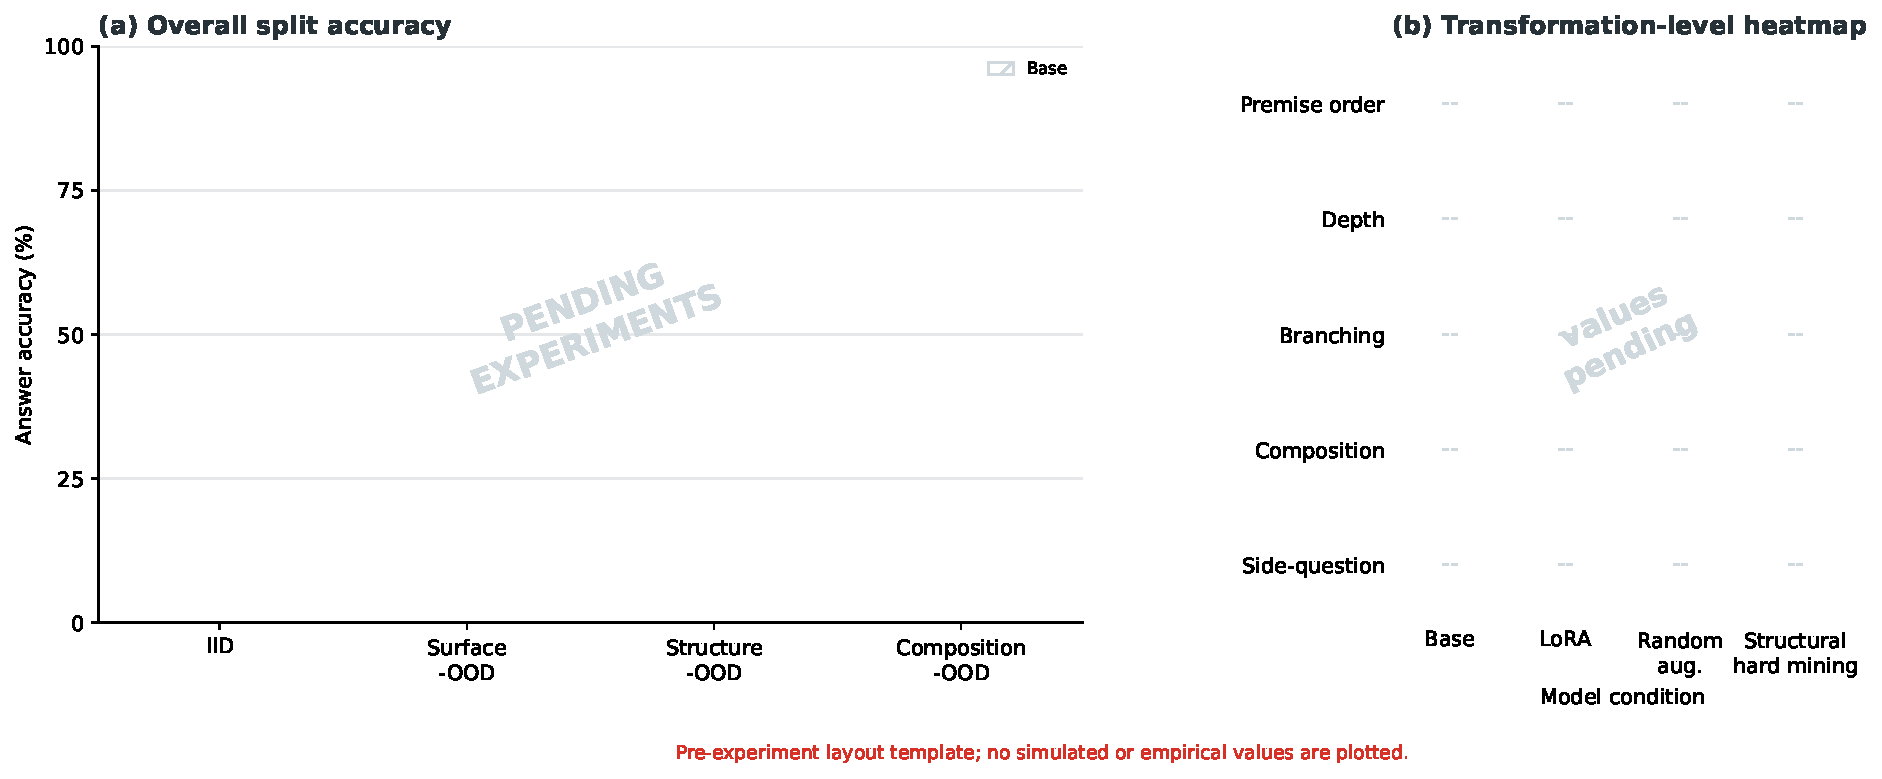
\includegraphics[width=\linewidth]{fig3_results_template.pdf}
  \caption{结构稳定性、结构迁移、错误预测和边界实验的结果图模板。正式数据出来前不填写数值。}
  \label{fig:results-zh}
\end{figure}

\section{适用边界}

将测试条件写成
\begin{equation}
\tau=(\mathcal G,\mathcal R,\mathcal Q,m,d),
\end{equation}
分别表示图分布、呈现分布、任务族、模型和解码条件。冻结 discovery 集得到的特征算法、标准化参数、模型规格和系数方向后，定义
\begin{equation}
V(\tau)=
\mathbf 1\{\text{方向一致}\}
\mathbf 1\{\text{预测优于最强对照}\}
\mathbf 1\{\text{校准通过}\}.
\end{equation}
规律的适用域为
\begin{equation}
\mathcal A=\{\tau:V(\tau)=1\}.
\end{equation}
边界实验一次只改变一个主要因素，并记录任务族、图分布、呈现规则、模型和干预条件。这样可以报告规律在哪些条件下成立，在哪些条件下失效。

\section{讨论与局限}

本文的稳定性定义只覆盖保持同一依赖图的呈现变化，不能代表所有形式的鲁棒性。迁移定义依赖严格的图族切分；若图族划分不充分，所谓未见结构可能只是换了表面词汇。依赖负担规律是任务层面的可观察预测，不直接揭示模型内部状态。稳定性与迁移之间的跨模型关系也不能单独证明因果关系。训练干预若只改善已见变体，应报告为局部适应而不是推理能力提升。

\section{结论}

本文将大语言模型推理中的两个问题分开：同一依赖图的结构稳定性，以及新依赖图上的结构迁移。稳定性使用同图条件保持率测量，迁移使用独立图族的规范呈现性能差距测量。研究进一步用依赖负担规律预测未见结构错误，并用适用域 $\mathcal A$、第二任务族和匹配干预确定其边界。最终结论将严格限制在实际支持的任务族、模型条件和结构范围内。

\appendix
\section{闭包求解器与有限反例的证明}
\label{app:proofs-zh}

形式化在 Lake 项目 \texttt{proof/StructRobust}，使用 Lean~4.35.0 的核心库，不依赖 mathlib。下面只写人读得懂的论证，并标出文件路径和定理名，不粘贴 tactic 脚本。每一条都是关于闭包求解器和有限反例的定理，不是对已训练模型的实测结论。

\subsection{闭包}
\label{app:closure-zh}

文件 \texttt{proof/StructRobust/StructRobust/Closure.lean}，定理 \texttt{closure\_fuel\_iff\_derives}。

前向链一轮把所有前提已满足的规则的结论加入已知集。势函数取「结论尚未出现的规则条数」。若一轮真正加入了新结论，势严格下降。势不超过规则条数，因此燃料不少于规则条数时计算到达不动点。不动点上，可推导的原子都已出现；反过来，闭包中的原子都可以按加入顺序写成确定子句推导。于是燃料足够时，成员关系就是确定子句闭包。推导只看规则是否属于规则集，不看列表顺序，所以规则集相同则推导关系相同（\texttt{derives\_rules\_congr}）。

\subsection{引理~\ref{lem:order-zh}}

文件 \texttt{proof/StructRobust/StructRobust/Operators.lean}。

顺序。\texttt{lemma1\_order\_preserves}：两个规则列表若作为集合相同，则查询可推导当且仅当在另一列表上可推导，求解器答案不变。\texttt{lemma1\_reorder\_stable}：把列表换成成员相同的列表不改事实集和查询，因此是稳定性变换。\texttt{stability\_preserves}：凡稳定性变换都保持求解器答案。

同义。\texttt{lemma1\_synonym\_denote}：句式包装只改包装层的编号，指称仍读出同一条规则。\texttt{lemma1\_synonym\_extract}：对列表逐条包装后再抽取，得到的规则列表与原列表相同。

歧义。取事实为空、规则 $\{0\}\to 1$、查询 $1$。空事实不能提供前提 $0$，唯一的规则又需要 $0$，所以任何原子都推不出（\texttt{derives\_amb\_false}）。删去前提后规则变成空前提推出 $1$，空前提立即触发，查询 $1$ 可推导（\texttt{derives\_dropped}）。\texttt{lemma1\_ambiguity\_changes} 记录答案由否变为是。若这次删前提是稳定性变换，答案必须保持，矛盾，故 \texttt{lemma1\_ambiguity\_not\_stability}。

换图。任务甲的规则是 $\{0\}\to 1$，任务乙的规则是 $\{0\}\to 2$。甲的规则不在乙的规则集中，两个规则集不同。稳定性变换要求规则集相同，故 \texttt{lemma1\_graph\_not\_stability}。

\subsection{引理~\ref{lem:gap-zh}}

文件 \texttt{proof/StructRobust/StructRobust/Counting.lean}。

把 $C=1$ 拆成 $(C,S)=(1,0)$ 与 $(1,1)$，把 $S=1$ 拆成 $(0,1)$ 与 $(1,1)$。两式相减，共同的 $(1,1)$ 消去，得到
\[
\#\{C=1\}-\#\{S=1\}=\#\{C=1,S=0\}-\#\{C=0,S=1\}
\]
（\texttt{lemma2\_count\_gap}）。两边乘以 $\#\{C=1\}$，并用整数分配律，得到
\[
\bigl(\#\{C=1\}-\#\{S=1\}\bigr)\cdot\#\{C=1\}
=\#\{C=1,S=0\}\cdot\#\{C=1\}-\#\{C=0,S=1\}\cdot\#\{C=1\}
\]
（\texttt{lemma2\_gap\_times\_correct}）。右边第一项是改口次数与规范做对次数的乘积，第二项是被救回的次数与规范做对次数的乘积。差距为零只说明改口次数等于被救回的次数。

构造两个列表（\texttt{lemma2\_same\_accuracy\_different\_sf}）。稳定列表是 $60$ 条 $(1,1)$ 接 $40$ 条 $(0,0)$。改口列表是 $30$ 条 $(1,1)$、$30$ 条 $(1,0)$、$30$ 条 $(0,1)$ 和 $10$ 条 $(0,0)$。两者长度都是 $100$，$C=1$ 与 $S=1$ 的次数都是 $60$，准确率都是 $60/100$。稳定列表的改口次数是 $0$，改口列表是 $30$。在 $C=1$ 的 $60$ 条上，条件改口比分别是 $0/60=0$ 与 $30/60$。

\subsection{引理~\ref{lem:worlds-zh}}

文件 \texttt{proof/StructRobust/StructRobust/Worlds.lean}，定理 \texttt{lemma3\_same\_transfer\_different\_sf}。

世界甲的见过列表是两条 $(C,S)=(1,1)$，没见过的规范正确标记是两个真值。世界乙的见过列表是一条 $(1,0)$ 和一条 $(1,1)$，没见过的规范正确标记同样是两个真值。两个世界的见过规范正确次数都是 $2$，没见过的规范正确次数都是 $2$，差都是 $0$。见过图上的改口次数，甲是 $0$，乙是 $1$，分母都是 $2$。因此规范迁移差相同，见过图上的改口计数不同。

\subsection{引理~\ref{lem:interaction-zh}}

文件 \texttt{proof/StructRobust/StructRobust/Interaction.lean}，定理 \texttt{lemma4\_interaction\_opposite}。

展开
\begin{align*}
I&=A_{\mathrm{sc}}-A_{\mathrm{ss}}-A_{\mathrm{uc}}+A_{\mathrm{us}},\\
J&=A_{\mathrm{ss}}-A_{\mathrm{us}}-A_{\mathrm{sc}}+A_{\mathrm{uc}}.
\end{align*}
对应项互为相反数，故 $I+J=0$，即 $I=-J$。这里的四个量是任意整数，不需要把它们解释成某次训练的准确率。

\subsection{引理~\ref{lem:inversion-zh}}

文件 \texttt{proof/StructRobust/StructRobust/Inversion.lean}。

逆序对按位置定义：前面的数大于后面的数就记一对。正序列表 $0,1,\ldots,m-1$ 中每个数都不大于它后面的数，逆序对数是 $0$（\texttt{lemma5\_canon\_inversions}）。完全倒序是 $m-1,\ldots,0$。对长度作归纳：空列表为 $0$；在长度为 $m$ 的倒序前面放上 $m$ 时，$m$ 大于后面每一个数，新增 $m$ 对，原有逆序对不变。于是二倍逆序对数满足 $2\cdot I(m+1)=2\cdot I(m)+2m$，而 $2m+m(m-1)=(m+1)m$，故 $I(m)=m(m-1)/2$（\texttt{lemma5\_reverse\_inversions}）。代入 $m=2$ 得 $1$，代入 $m=3$ 得 $3$（\texttt{lemma5\_reverse\_two}、\texttt{lemma5\_reverse\_three}）。$1\neq 3$（\texttt{lemma5\_reverse\_two\_ne\_three}）。因此核心规则条数为 $2$ 与 $3$ 时，完全倒序的逆序对数不同。这是计数，不是对模型输出的测量。

\subsection{定理~\ref{thm:main-zh} 的正支}

文件 \texttt{proof/StructRobust/StructRobust/Main.lean}。

抽取把每条包装句还原成它所指的规则。$f$ 判定查询是否属于抽取出的规则集的闭包。若两个包装列表抽出的规则集相同，则闭包成员关系相同，所以 $f$ 在这两个写法上同时为真或同时为假，并且等于该规则集上的求解器答案（\texttt{main\_positive\_orbit}）。顺序只重排包装列表的成员，抽出的规则集不变（\texttt{main\_positive\_reorder}）。同义包装不改变抽取（\texttt{main\_positive\_synonym}，用到 \texttt{lemma1\_synonym\_extract}）。因此，只要规范写法使 $f$ 为真，同一轨道上的变换写法也使 $f$ 为真（\texttt{main\_positive\_finite\_ss}）。对有限题单逐条使用同一论证，规范做对的题全部在变换后做对（\texttt{main\_positive\_finite\_ss\_all}）。若一道没见过的题的规范抽取已经使求解器接受查询，则规范写法和规则集相同的等价写法都使 $f$ 为真（\texttt{main\_positive\_unseen}）。

\subsection{定理~\ref{thm:main-zh} 的反支}

同一文件。见过图的写法用标签区分：事实是 $[0]$，规则是 $\{0\}\to 1$，查询是 $1$。前提 $0$ 是事实，故查询可推导，求解器接受。函数在每一个见过标签上输出真，与求解器一致（\texttt{main\_negative\_seen\_correct}），并且不随标签改变（\texttt{main\_negative\_seen\_stable}）。没见过的那一道题事实为空，规则是空前提推出 $2$，查询是 $2$。空前提立即触发，求解器接受；该函数输出假，与求解器不一致（\texttt{main\_negative\_unseen\_incorrect}）。见过图的规则 $\{0\}\to 1$ 不属于没见过题的规则集，两个规则集不同（\texttt{main\_negative\_disjoint}）。因此见过图上的稳定与正确，推不出这道不相交的没见过题正确。

\begin{thebibliography}{99}
\bibitem{hupkes2020} D. Hupkes, V. Dankers, M. Mul, and E. Bruni. Compositionality Decomposed: How Do Neural Networks Generalise? JAIR, 2020.
\bibitem{oren2020} J. Oren et al. Improving Compositional Generalization in Semantic Parsing. Findings of EMNLP, 2020.
\bibitem{herzig2021} J. Herzig and J. Berant. Span-based Semantic Parsing for Compositional Generalization. ACL-IJCNLP, 2021.
\bibitem{qiu2022} L. Qiu et al. Evaluating the Impact of Model Scale for Compositional Generalization in Semantic Parsing. EMNLP, 2022.
\bibitem{mirzadeh2024} I. Mirzadeh et al. GSM-Symbolic: Understanding the Limitations of Mathematical Reasoning in Large Language Models. arXiv, 2024.
\bibitem{li2024} Q. Li et al. GSM-Plus: A Comprehensive Benchmark for Evaluating the Robustness of LLMs as Mathematical Problem Solvers. ACL, 2024.
\bibitem{shi2023} F. Shi et al. Large Language Models Can Be Easily Distracted by Irrelevant Context. arXiv, 2023.
\bibitem{liu2024} N. F. Liu et al. Lost in the Middle: How Language Models Use Long Contexts. TACL, 2024.
\bibitem{zhou2024} Z. Zhou et al. Can Language Models Perform Robust Reasoning in Chain-of-thought Prompting with Noisy Rationales? NeurIPS, 2024.
\bibitem{paul2024} D. Paul et al. Making Reasoning Matter: Measuring and Improving Faithfulness of Chain-of-Thought Reasoning. Findings of EMNLP, 2024.
\bibitem{press2023} O. Press et al. Measuring and Narrowing the Compositionality Gap in Language Models. Findings of EMNLP, 2023.
\bibitem{jia2017} R. Jia and P. Liang. Adversarial Examples for Evaluating Reading Comprehension Systems. EMNLP, 2017.
\bibitem{hu2022} E. J. Hu et al. LoRA: Low-Rank Adaptation of Large Language Models. ICLR, 2022.
\bibitem{dettmers2023} T. Dettmers et al. QLoRA: Efficient Finetuning of Quantized Language Models. NeurIPS, 2023.
\bibitem{pereira2021} J. Pereira et al. Targeted Adversarial Training for Natural Language Understanding. NAACL, 2021.
\end{thebibliography}
\end{document}
